% !TeX TXS-program:compile = txs:///pdflatex/[--shell-escape]

\documentclass[12pt,a4paper,english]{article}
\usepackage{geometry,graphicx}
\usepackage[hidelinks]{hyperref}
\usepackage[parfill]{parskip}
\usepackage[super]{nth}
\usepackage{listings}
\usepackage{float}
\usepackage{xcolor}
\usepackage{tikz}
\usetikzlibrary{arrows.meta}

\graphicspath{ {../sprites/} }

\geometry{
	a4paper,
	total={180mm,252mm},
	left=15mm,
	top=25mm,
	footnotesep=0.8cm,
}

\newcommand{\cod}[1]{{\fontfamily{qcr}\selectfont{\small#1}}}

\begin{document}

\begin{titlepage}
	\begin{center}
		\vspace*{1cm}
		
		{\LARGE\textbf{Exercise 1 - Distributed Systems}}
		
		\vspace{0.2cm}
		
		{\large A Naive View}
		
		\vspace{1cm}
		
		{\Large Spencer Johnson (spencerjames.johnson)}
		
		\vfill
		
		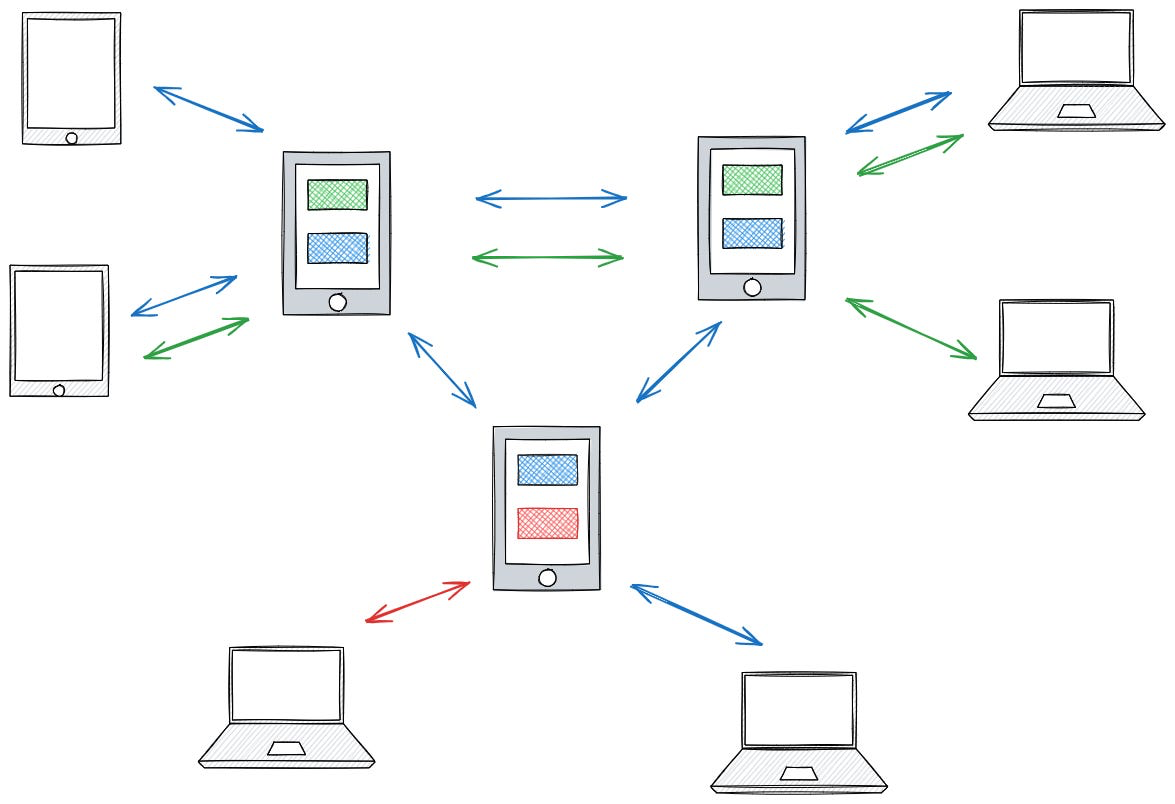
\includegraphics[width=0.55\textwidth]{cover.png}
		
		\vfill
		
		\begin{abstract}
			This report describes a socket-based distributed counter system. The objective is to share an integer variable between several server processes without using semaphores, shared memory, message queues, or other IPC mechanisms. The implemented solution uses socket frames and a token ring to control when each server can read or update the shared value.
		\end{abstract}
		
		\vfill
		
		
\includegraphics[width=0.25\textwidth]{lasalle.png}
		
		\vspace{1cm}
		
		Distributed Systems
		
		\vspace{0.2cm}
		
		La Salle URL - Barcelona, Spain
		
		\vspace{0.2cm}
		
		\nth{2} October 2026
		
		\vspace*{0.5cm}
	\end{center}
\end{titlepage}

\newpage

\tableofcontents

\newpage

\section{Introduction}

The goal of this exercise is to share one integer variable between \cod{N} server processes. The servers are only allowed to communicate through sockets. Each server has one behavior selected at startup: read-write or read-only.

The integer value starts at \cod{0}. Read-write servers read the current value and update it with \cod{value + 1}. Read-only servers only read the current value. Each server performs this behavior for a fixed number of turns.

\section{System Architecture}

\subsection{Processes Overview}

\begin{itemize}
	\item \textbf{menu.js}: Starts all servers and builds the ring configuration.
	\item \textbf{server.js}: Represents one server in the distributed system.
\end{itemize}

\subsection{Server Functionality}

\begin{itemize}
	\item \textbf{Read-write server}: Reads the value and updates it by one.
	\item \textbf{Read-only server}: Reads the value without changing it.
\end{itemize}

\subsection{Ring Structure}

\begin{figure}[H]
	\centering
	\fbox{
		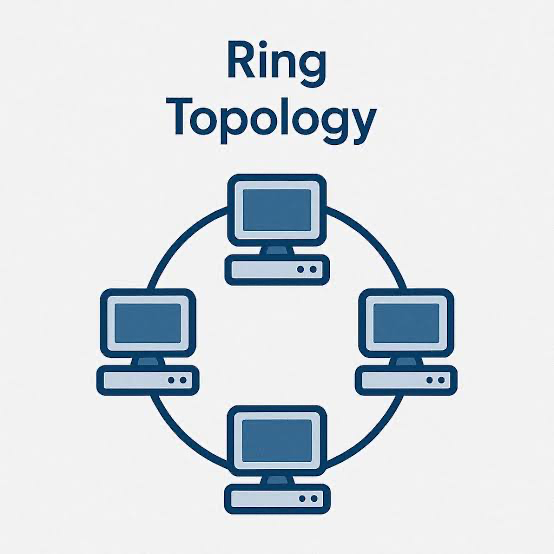
\includegraphics[width=0.30\textwidth]{ring_topology.png}
	}
	\caption{Ring topology used for token passing between servers.}
	\label{fig:ring-topology}
\end{figure}

Each server knows the previous server and the next server. The token moves from one server to the next. A server can only perform its turn after receiving the token.

\newpage

\section{Communication Protocol}

The system communicates using simple socket frames.

\begin{itemize}
	\item \cod{READ}: Returns the current local value.
	\item \cod{UPDATE <value>}: Updates the current local value.
	\item \cod{TOKEN}: Gives a server permission to take its turn.
\end{itemize}

\cod{READ} and \cod{UPDATE <value>} are the two operations on the shared variable. The \cod{TOKEN} frame is used only to control turn order.

\section{Algorithm}

\subsection{Algorithm 1: Neighbor Read}

\begin{figure}[H]
	\centering
	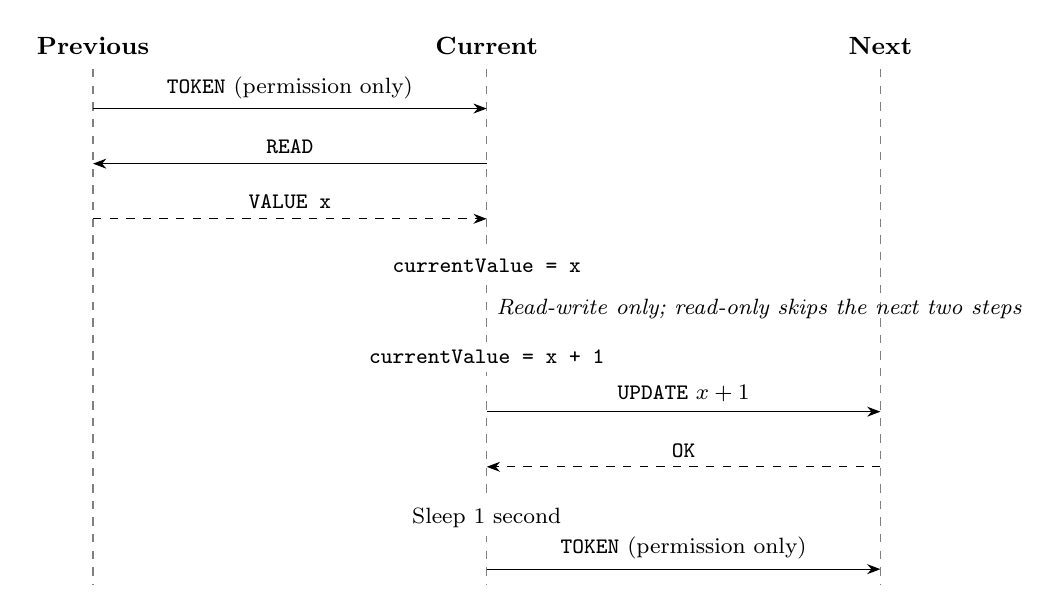
\begin{tikzpicture}[font=\footnotesize, >=Stealth]
		\node[font=\small\bfseries] at (0,0) {Previous};
		\node[font=\small\bfseries] at (5,0) {Current};
		\node[font=\small\bfseries] at (10,0) {Next};
		\foreach \x in {0,5,10} {
			\draw[dashed, gray] (\x,-0.3) -- (\x,-6.85);
		}

		\draw[->] (0,-0.8) -- node[above] {\texttt{TOKEN} (permission only)} (5,-0.8);
		\draw[->] (5,-1.5) -- node[above] {\texttt{READ}} (0,-1.5);
		\draw[->, dashed] (0,-2.2) -- node[above] {\texttt{VALUE x}} (5,-2.2);
		\node[fill=white, inner sep=3pt] at (5,-2.8) {\texttt{currentValue = x}};

		\node[font=\footnotesize\itshape, anchor=west] at (5,-3.35) {Read-write only; read-only skips the next two steps};
		\node[fill=white, inner sep=3pt] at (5,-3.95) {\texttt{currentValue = x + 1}};
		\draw[->] (5,-4.65) -- node[above] {\texttt{UPDATE} $x+1$} (10,-4.65);
		\draw[->, dashed] (10,-5.35) -- node[above] {\texttt{OK}} (5,-5.35);

		\node[fill=white, inner sep=3pt] at (5,-6) {Sleep 1 second};
		\draw[->] (5,-6.65) -- node[above] {\texttt{TOKEN} (permission only)} (10,-6.65);
	\end{tikzpicture}
	\caption{One active turn in Algorithm 1. \cod{UPDATE} carries the computed integer $x+1$. Token acknowledgements are omitted for clarity.}
	\label{fig:algorithm-one-sequence}
\end{figure}

\subsection{Algorithm 2: Broadcast Update}

\begin{figure}[H]
\centering
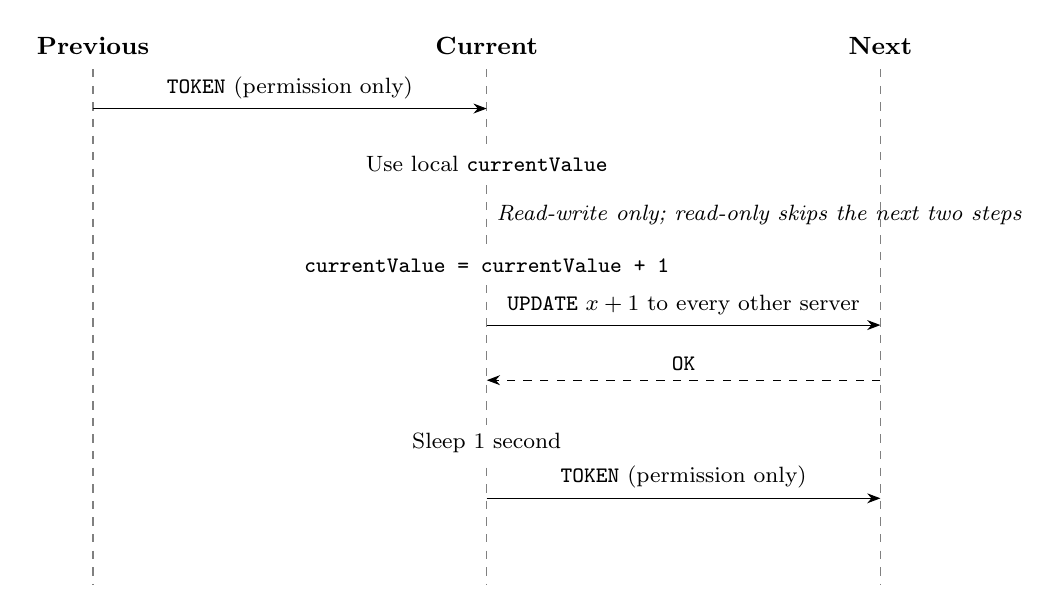
\begin{tikzpicture}[font=\footnotesize, >=Stealth]
	\node[font=\small\bfseries] at (0,0) {Previous};
	\node[font=\small\bfseries] at (5,0) {Current};
	\node[font=\small\bfseries] at (10,0) {Next};
	\foreach \x in {0,5,10} {
		\draw[dashed, gray] (\x,-0.3) -- (\x,-6.85);
	}

	\draw[->] (0,-0.8) -- node[above] {\texttt{TOKEN} (permission only)} (5,-0.8);
	\node[fill=white, inner sep=3pt] at (5,-1.5) {Use local \texttt{currentValue}};

	\node[font=\footnotesize\itshape, anchor=west] at (5,-2.15) {Read-write only; read-only skips the next two steps};
	\node[fill=white, inner sep=3pt] at (5,-2.8) {\texttt{currentValue = currentValue + 1}};
	\draw[->] (5,-3.55) -- node[above] {\texttt{UPDATE} $x+1$ to every other server} (10,-3.55);
	\draw[->, dashed] (10,-4.25) -- node[above] {\texttt{OK}} (5,-4.25);

	\node[fill=white, inner sep=3pt] at (5,-5.05) {Sleep 1 second};
	\draw[->] (5,-5.75) -- node[above] {\texttt{TOKEN} (permission only)} (10,-5.75);
\end{tikzpicture}
\caption{One active turn in Algorithm 2. A read-write server broadcasts its new local value before passing the token.}
\label{fig:algorithm-two-sequence}
\end{figure}

\newpage

\section{Results}

\subsection{Testing Configurations}

\begin{itemize}
	\item 100 servers.
	\item 75 read-write servers and 25 read-only servers.
	\item 10 turns per server, with a 1000ms sleep during every turn.
	\item Algorithm 1 and Algorithm 2 were run separately using the same configuration.
\end{itemize}

\subsection{Performance Overhead}

The timing results were collected from the terminal output. Each completed turn records the UTC timestamp, server port, server type, turn number, read value, and local value:

\begin{verbatim}
2026-10-13T23:55:55.012Z | Server 5002 |
ReadWrite | Turn 1 | Read 0 | Value 1
\end{verbatim}

The execution time was measured from the first turn of server \cod{5002} until server \cod{5001} completed its tenth turn. Every 100-server execution contains 1000 required one-second sleeps, so the fixed 1000 seconds were subtracted from the measurements below. Both tests finished with the expected value of \cod{750}, since 75 read-write servers each incremented the value 10 times.

\begin{table}[H]
\centering
\begin{tabular}{|l|c|c|c|}
\hline
Algorithm & Servers & Final value & Time excluding sleep (s) \\
\hline
Algorithm 1: Neighbor Read & 100 & 750 & 6.991 \\
\hline
Algorithm 2: Broadcast Update & 100 & 750 & 42.926 \\
\hline
\end{tabular}
\caption{Communication and processing time after removing the required sleep time.}
\label{tab:performance-results}
\end{table}

\begin{figure}[H]
\centering
\fbox{
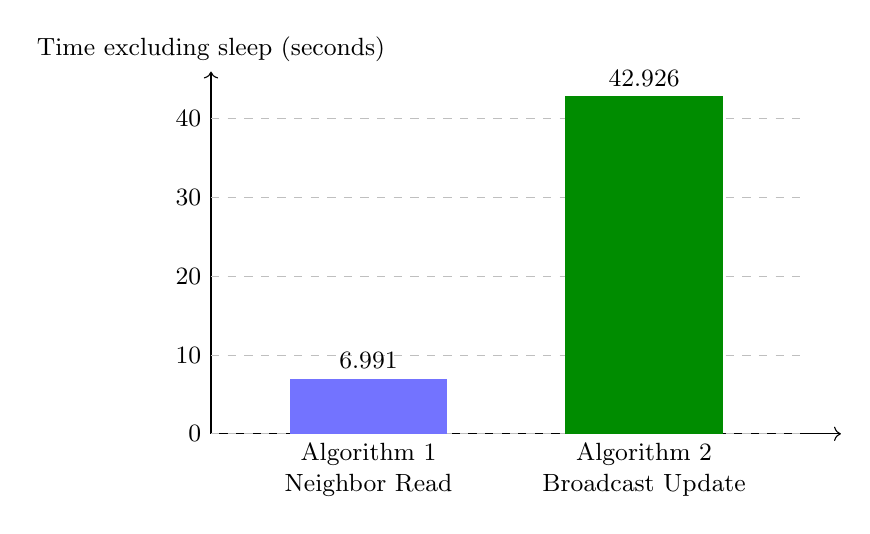
\begin{tikzpicture}[x=1cm,y=0.10cm,font=\small]
\draw[->] (0,0) -- (0,46) node[above] {Time excluding sleep (seconds)};
\draw[->] (0,0) -- (8,0);

\foreach \y in {0,10,20,30,40} {
	\draw[dashed, gray!50] (0,\y) -- (7.5,\y);
	\node[left] at (0,\y) {\y};
}

\fill[blue!55] (1,0) rectangle (3,6.991);
\fill[green!55!black] (4.5,0) rectangle (6.5,42.926);
\node[above] at (2,6.991) {6.991};
\node[above] at (5.5,42.926) {42.926};
\node[align=center, below] at (2,0) {Algorithm 1\\Neighbor Read};
\node[align=center, below] at (5.5,0) {Algorithm 2\\Broadcast Update};
\end{tikzpicture}
}
\caption{Communication and processing time for the completed 100-server tests, excluding the required sleep time.}
\label{fig:performance-comparison}
\end{figure}

After removing the required sleep time, Algorithm 2 took 35.935 seconds longer than Algorithm 1. The extra time comes from each read-write server sending an \cod{UPDATE} frame to every other server.

\subsection{Large Ring Test}

The 750-server tests completed one full rotation before being stopped. To compare the ring sizes, the required sleep time was removed from the duration of that first rotation. The 100-server test used 75 read-write servers, while the 750-server test used 20 read-write servers.

\begin{figure}[H]
\centering
\fbox{
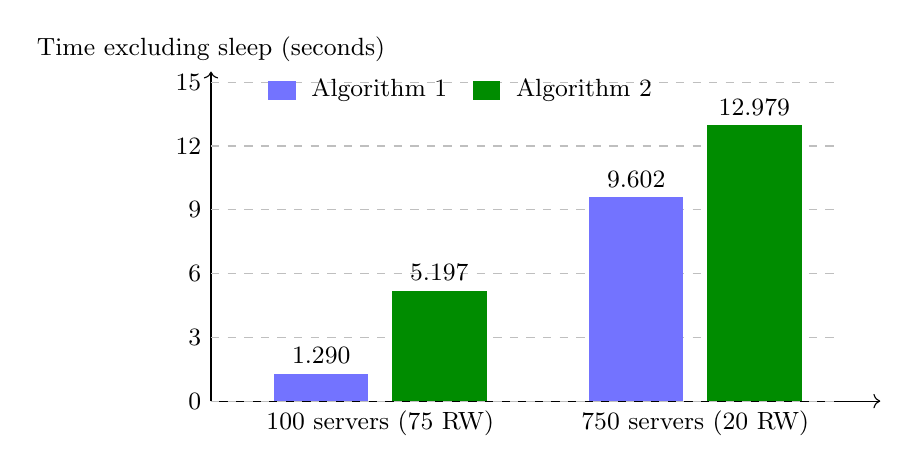
\begin{tikzpicture}[x=1cm,y=0.27cm,font=\small]
\draw[->] (0,0) -- (0,15.5) node[above] {Time excluding sleep (seconds)};
\draw[->] (0,0) -- (8.5,0);

\foreach \y in {0,3,6,9,12,15} {
	\draw[dashed, gray!50] (0,\y) -- (8,\y);
	\node[left] at (0,\y) {\y};
}

\fill[blue!55] (0.8,0) rectangle (2.0,1.290);
\fill[green!55!black] (2.3,0) rectangle (3.5,5.197);
\fill[blue!55] (4.8,0) rectangle (6.0,9.602);
\fill[green!55!black] (6.3,0) rectangle (7.5,12.979);

\node[above] at (1.4,1.290) {1.290};
\node[above] at (2.9,5.197) {5.197};
\node[above] at (5.4,9.602) {9.602};
\node[above] at (6.9,12.979) {12.979};

\node[below] at (2.15,0) {100 servers (75 RW)};
\node[below] at (6.15,0) {750 servers (20 RW)};
\node[fill=blue!55, minimum width=0.35cm, minimum height=0.22cm] at (0.9,14.6) {};
\node[anchor=west] at (1.15,14.6) {Algorithm 1};
\node[fill=green!55!black, minimum width=0.35cm, minimum height=0.22cm] at (3.5,14.6) {};
\node[anchor=west] at (3.75,14.6) {Algorithm 2};
\end{tikzpicture}
}
\caption{Communication and processing overhead during one full ring rotation. The 750-server result covers the completed first rotation only.}
\label{fig:large-ring-test}
\end{figure}

\section{Limitations}

\begin{itemize}
	\item The token ring depends on all servers staying alive.
	\item If one server fails, the token may stop moving.
	\item Adding servers during execution is not currently supported.
	\item Larger rings increase the time needed for the token to return to the same server.
\end{itemize}

\section{Adding Servers Mid-Run}

To add servers during execution, the ring would need a way to safely update neighbor information. A joining server would need to be inserted between two existing servers without losing the token or breaking the current socket communication.

This would require extra control frames for joining, leaving, and updating neighbor addresses. It would also make the algorithm more complex because every server would need to agree on the new ring structure.

\section{Conclusion}

The implemented system follows the assignment restrictions by using sockets for communication and avoiding shared memory, semaphores, message queues, and other IPC mechanisms. The token ring provides a simple way to control access to the shared integer, while the two algorithm versions allow performance comparison between neighbor-based reading and broadcast-based updating.

\end{document}
